%!TEX TS-program = pdflatex
%!TEX root = progetto_finale.tex
%!TEX encoding = UTF-8 Unicode

\chapter{Automi}\label{automi_appendix}
  
\begin{figure}[htbp]
	\centering
	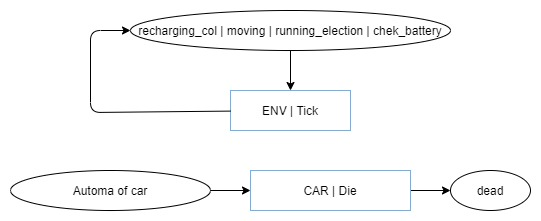
\includegraphics[width=13cm]{automa_macchina_global_events.jpg}
	\caption{Eventi globali automi macchina}
	\label{fig:automi_macchina_various}
\end{figure}

\begin{figure}[htbp]
	\centering
	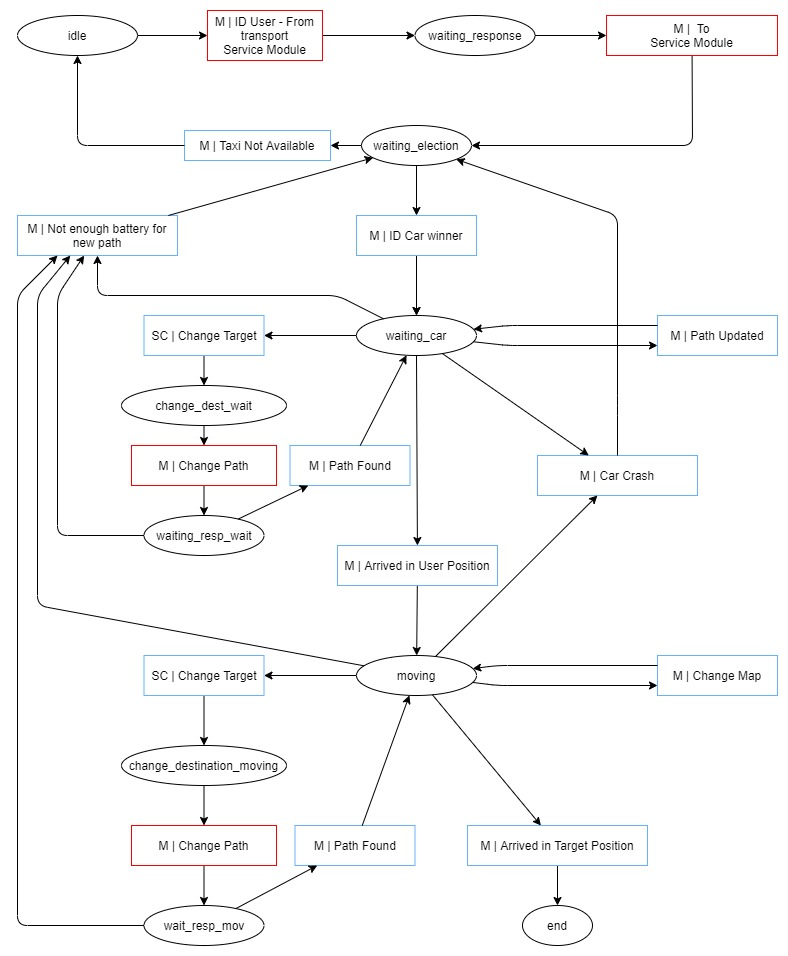
\includegraphics[width=14cm]{automa_utente.jpg}
	\caption{Rappresentazione degli stati possibili dell'entità utente.}
	\label{fig:automa_utente}
\end{figure}

\begin{figure}[htbp]
	\centering
	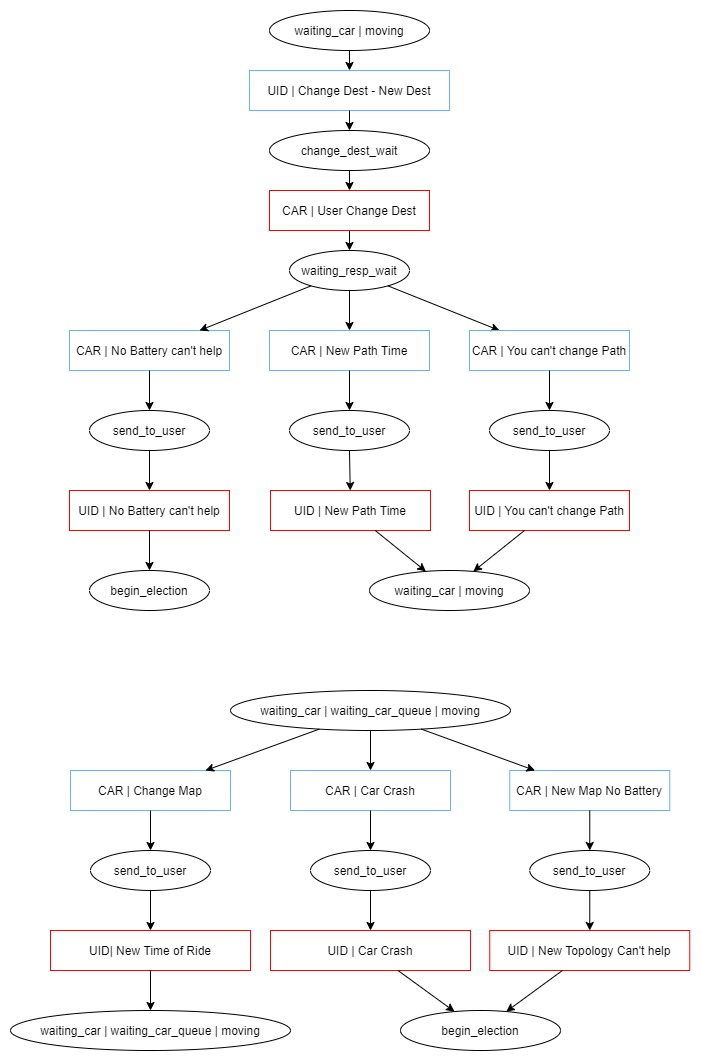
\includegraphics[width=13cm]{automa_app_utente_stati.jpg}
	\caption{Rappresentazione della gestione eventi dell'applicazione utente.}
	\label{fig:automa_app_utente_stati}
\end{figure}

\begin{figure}[htbp]
	\centering
	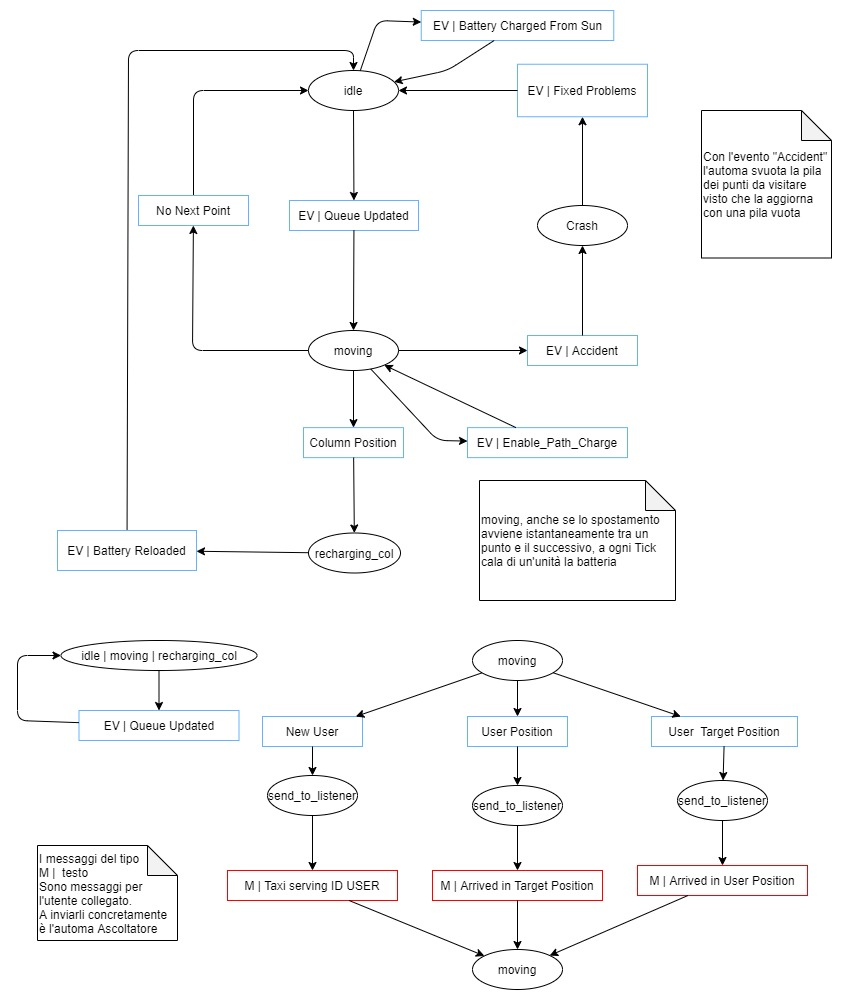
\includegraphics[width=14cm]{automa_macchina_moving.jpg}
	\caption{Rappresentazione degli stati macchina in servizio}
	\label{fig:automa_moving}
\end{figure}

\begin{figure}[htbp]
	\centering
	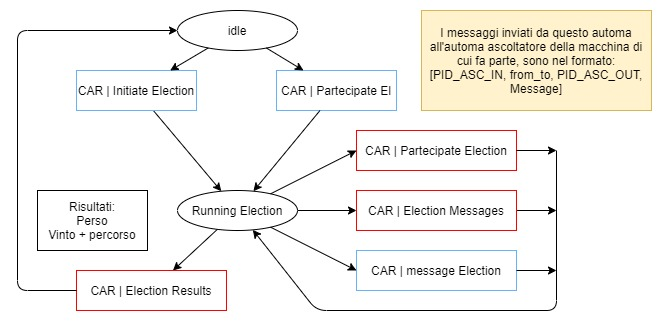
\includegraphics[width=14cm]{automa_macchina_elezione.jpg}
	\caption{Rappresentazione degli stati macchina - elezione}
	\label{fig:automa_elezione}
\end{figure}

\begin{figure}[htbp]
	\centering
	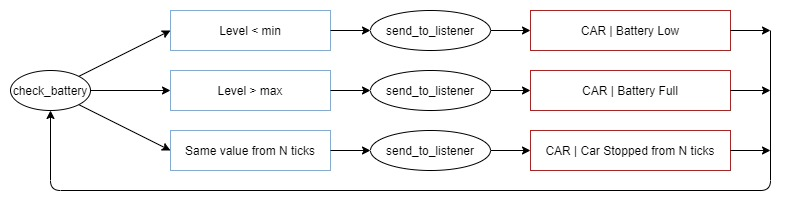
\includegraphics[width=14cm]{automa_macchina_batteria.jpg}
	\caption{Rappresentazione degli stati macchina - batteria}
	\label{fig:automa_batteria}
\end{figure}

\begin{figure}[htbp]
	\centering
	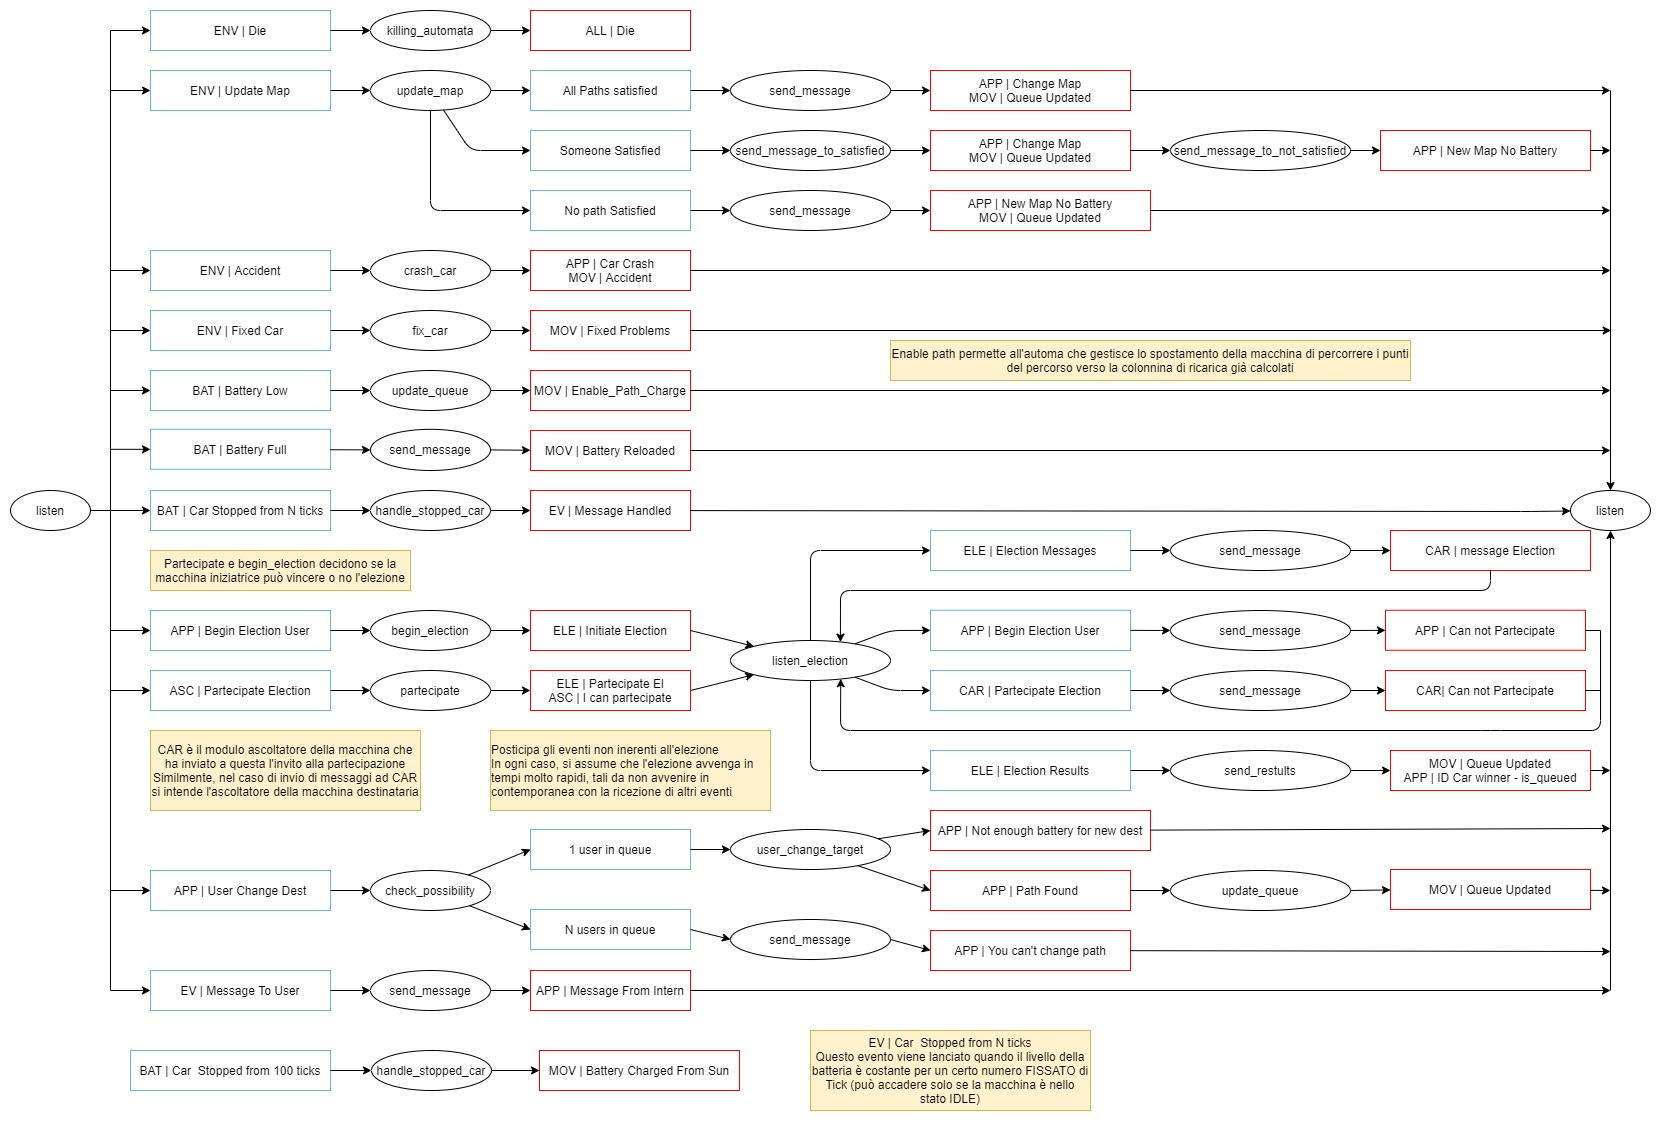
\includegraphics[width=19.5cm, angle = 90]{automa_macchina_ascoltatore.jpg}
	\caption{Rappresentazione degli stati macchina - listener}
	\label{fig:automa_listener}
\end{figure}

\chapter{Messaggi Scambiati}\label{messaggi_scambiati_appendix}

\begin{figure}[htbp]
	\centering
	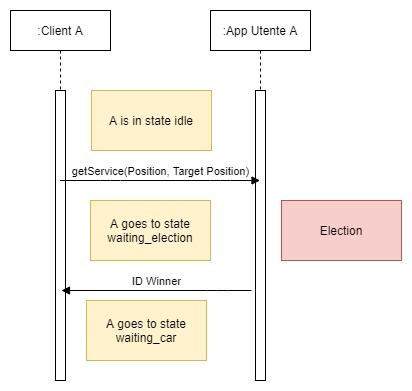
\includegraphics[width=13cm]{messaggi_utente_request_car.jpg}
	\caption{Messaggi scambiati per la richiesta di un trasporto.}
	\label{fig:messaggi_utente_request_car}
\end{figure}

\begin{figure}[htbp]
	\centering
	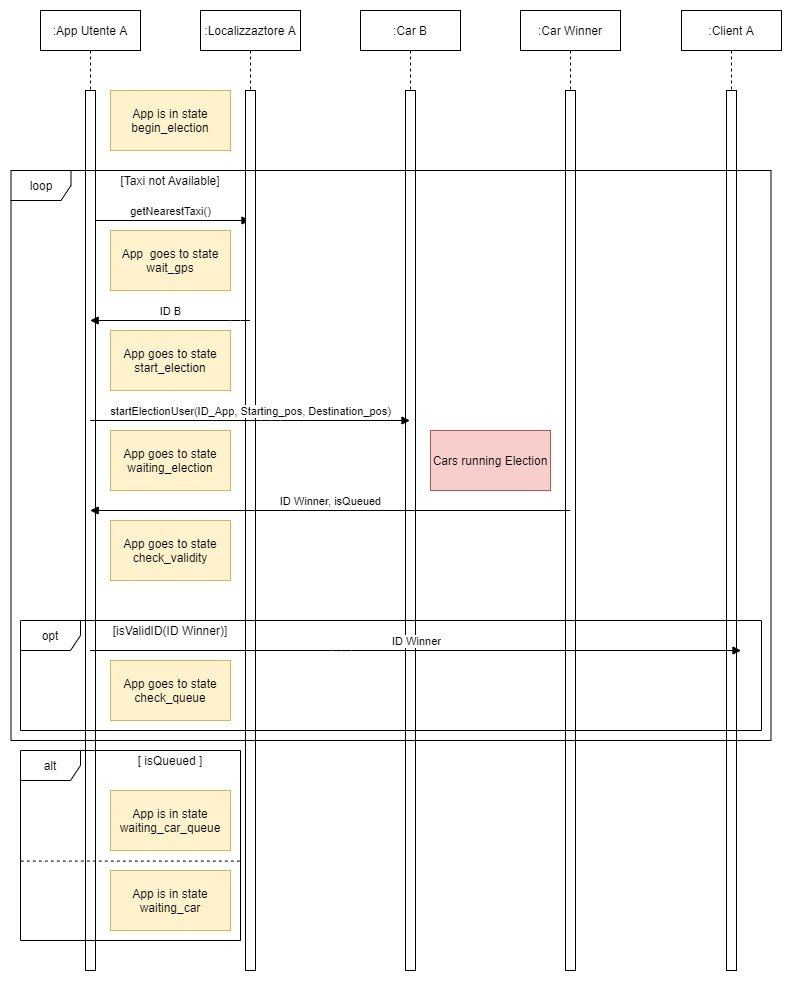
\includegraphics[width=14cm]{messaggi_app_utente_elezione.jpg}
	\caption{Messaggi scambiati dall'app dell'utente per l'elezione.}
	\label{fig:messaggi_app_utente_elezione}
\end{figure}

\begin{figure}[htbp]
	\centering
	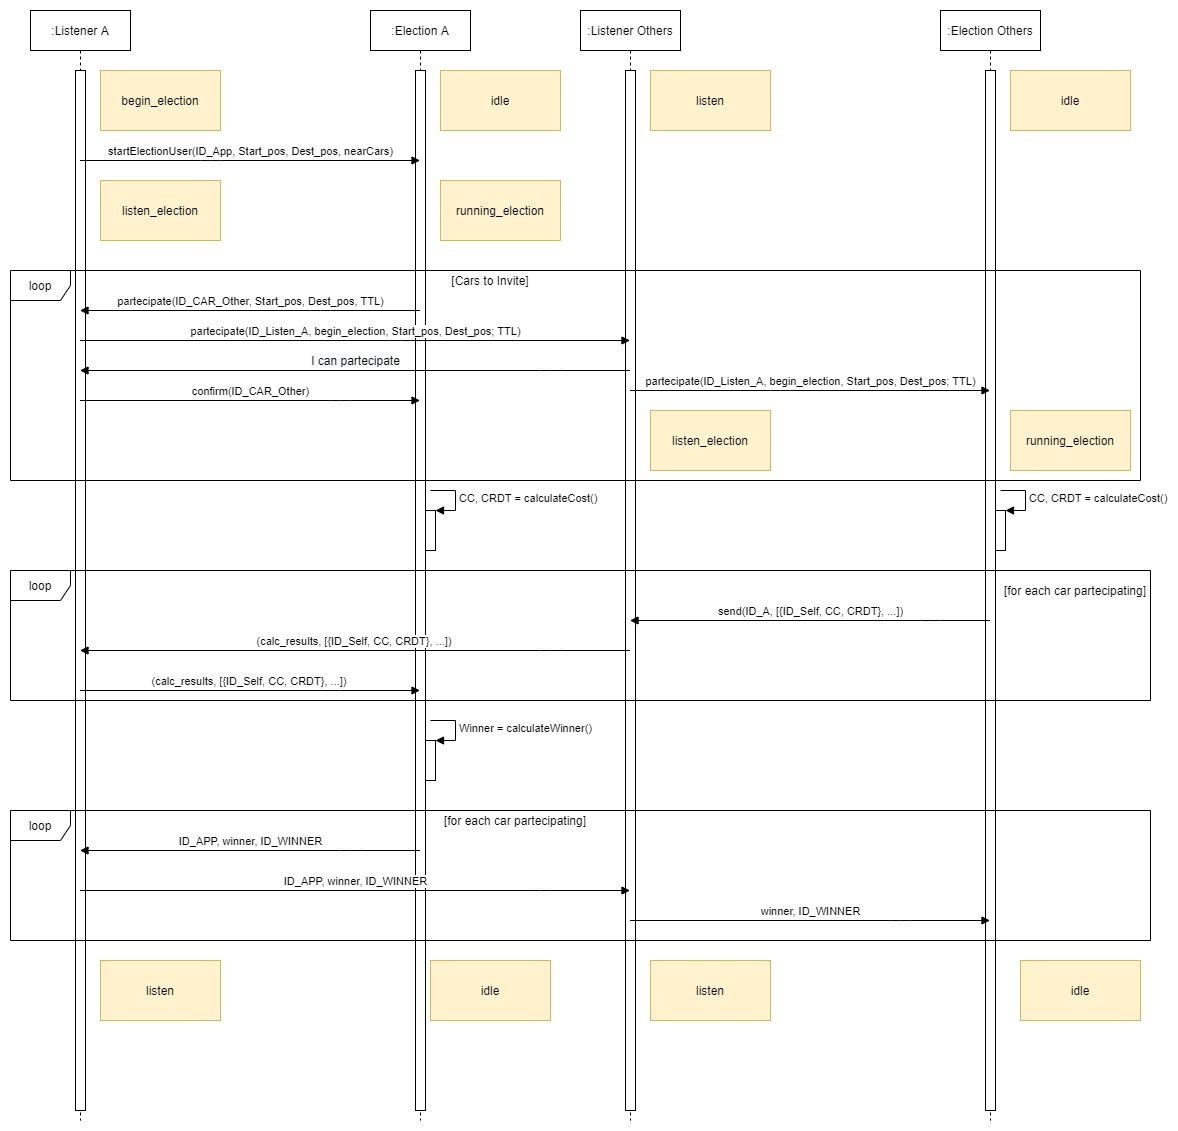
\includegraphics[width=14cm]{messaggi_macchina_iniziatore_elezione.jpg}
	\caption{Messaggi scambiati dalla macchina per l'elezione.}
	\label{fig:messaggi_macchina_iniziatore_elezione}
\end{figure}

\begin{figure}[htbp]
	\centering
	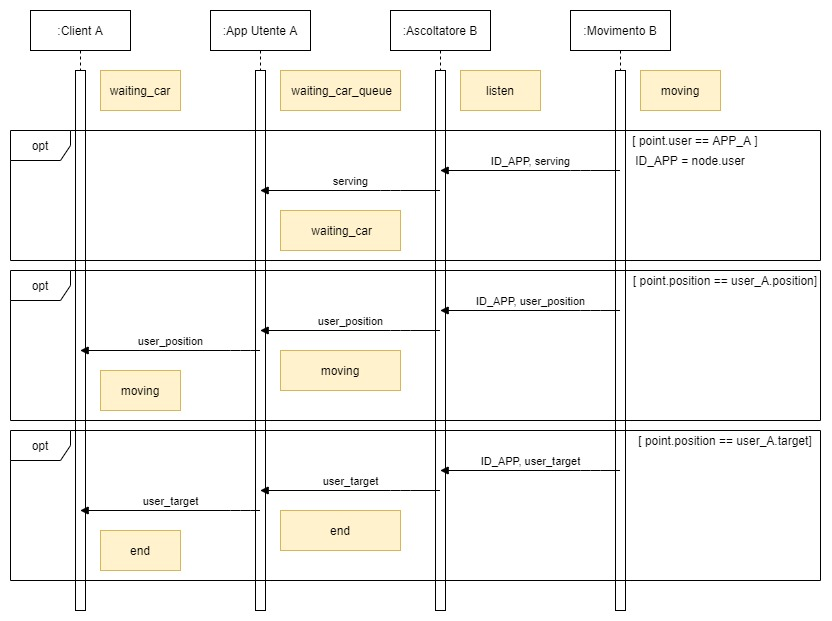
\includegraphics[width=14cm]{messaggi_utente_trasporto.jpg}
	\caption{Messaggi scambiati per il trasporto dell'utente.}
	\label{fig:messaggi_utente_trasporto}
\end{figure}

\begin{figure}[htbp]
	\centering
	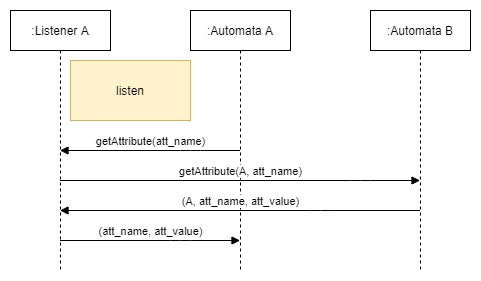
\includegraphics[width=13cm]{messaggi_macchina_get_attribute.jpg}
	\caption{Messaggi scambiati per l'ottenimento dei dati da automi interni.}
	\label{fig:messaggi_macchina_get_attribute}
\end{figure}

\begin{figure}[htbp]
	\centering
	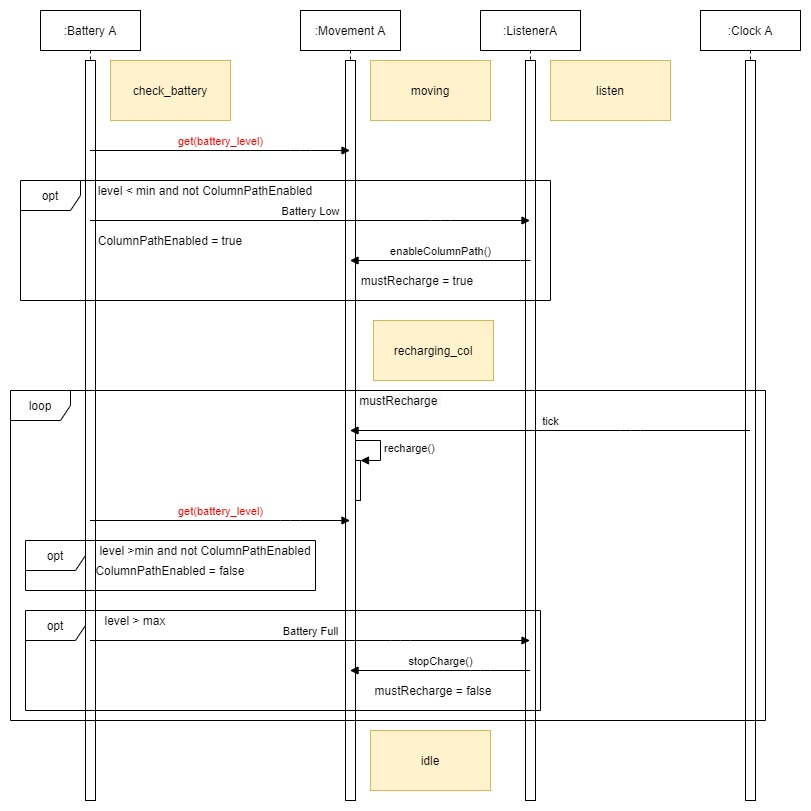
\includegraphics[width=13cm]{messaggi_macchina_batteria.jpg}
	\caption{Messaggi scambiati se la batteria della macchina è bassa.}
	\label{fig:messaggi_macchina_batteria}
\end{figure}

\begin{figure}[htbp]
	\centering
	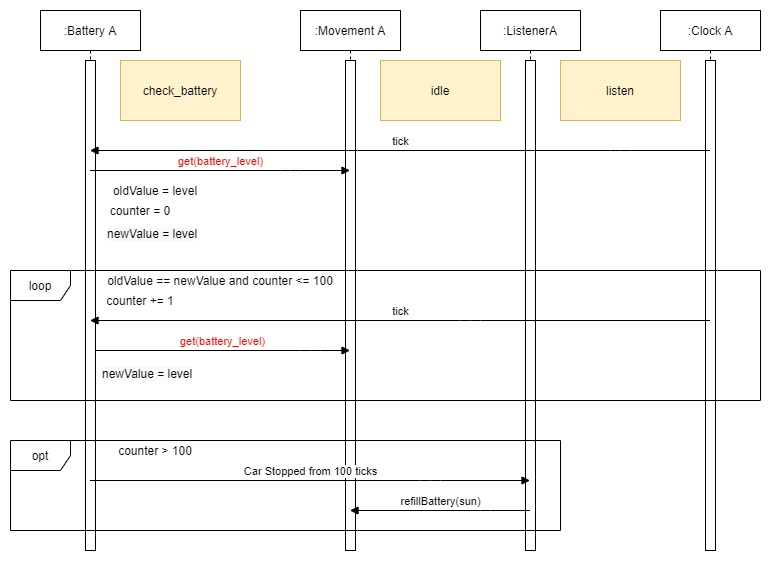
\includegraphics[width=13cm]{messaggi_macchina_pannelli_solari.jpg}
	\caption{Messaggi scambiati per la ricarica solare.}
	\label{fig:messaggi_macchina_pannelli_solari}
\end{figure}

\begin{figure}[htbp]
	\centering
	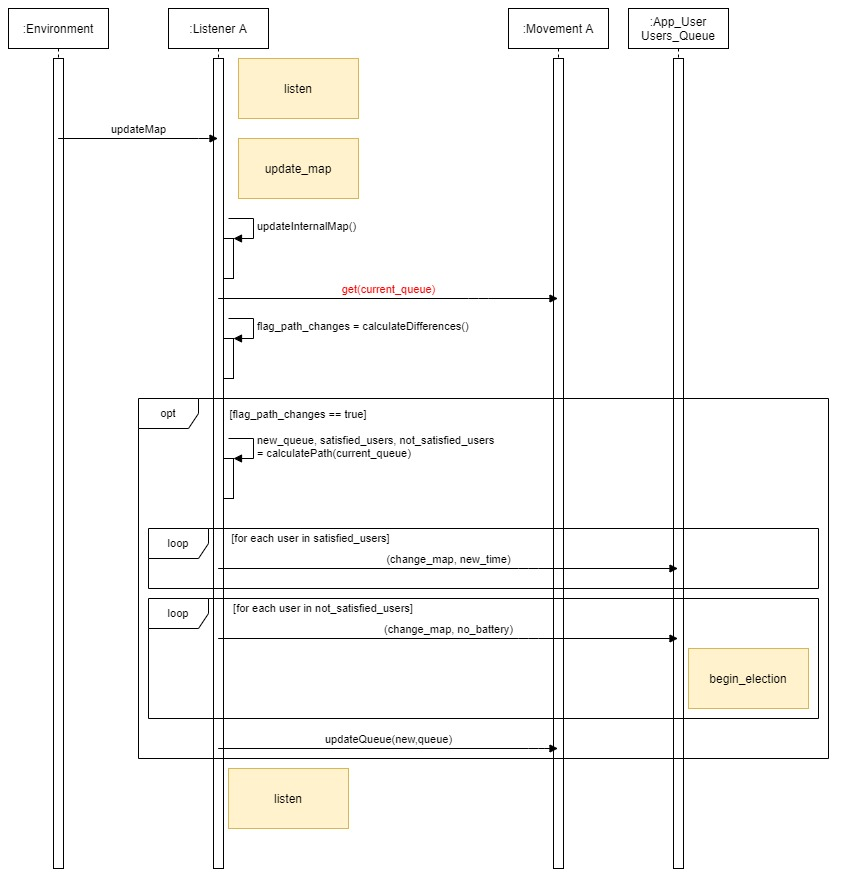
\includegraphics[width=13cm]{messaggi_macchina_update_map.jpg}
	\caption{Messaggi scambiati nell'aggiornamento della mappa.}
	\label{fig:messaggi_macchina_update_map}
\end{figure}

\begin{figure}[htbp]
	\centering
	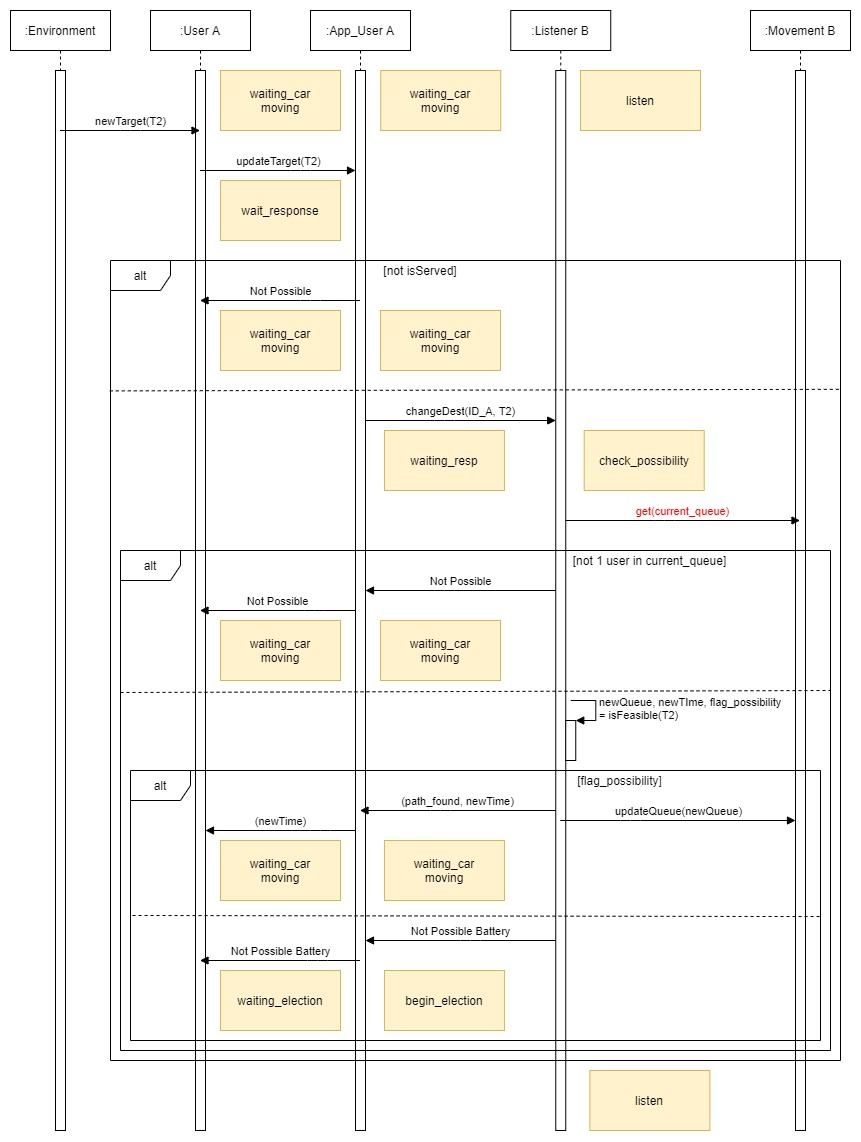
\includegraphics[width=13cm]{messaggi_utente_cambio_destinazione.jpg}
	\caption{Messaggi scambiati nel cambio destinazione dell'utente.}
	\label{fig:messaggi_utente_cambio_destinazione}
\end{figure}

\begin{figure}[htbp]
	\centering
	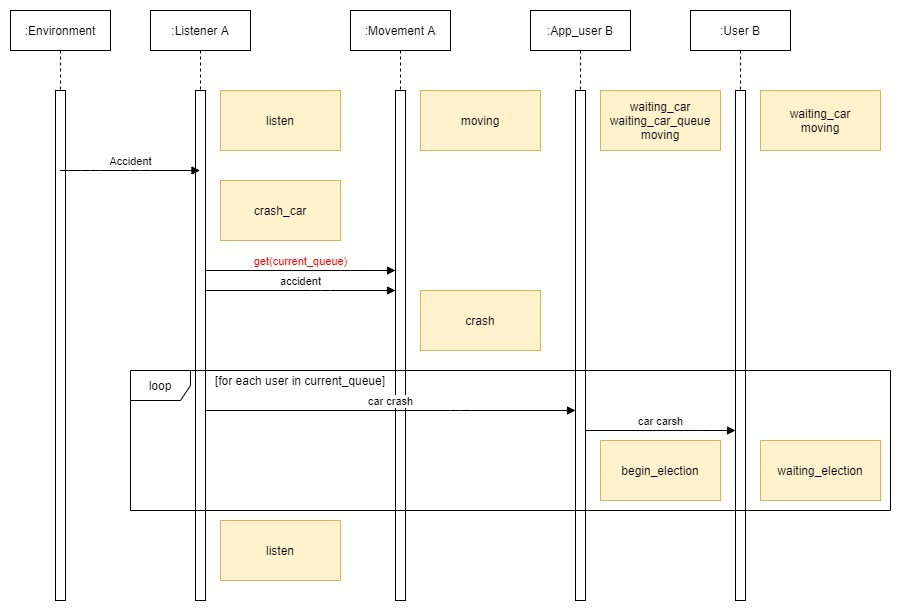
\includegraphics[width=13cm]{messaggi_macchina_incidente.jpg}
	\caption{Messaggi scambiati nel caso di un incidente.}
	\label{fig:messaggi_macchina_incidente}
\end{figure}

\begin{figure}[htbp]
	\centering
	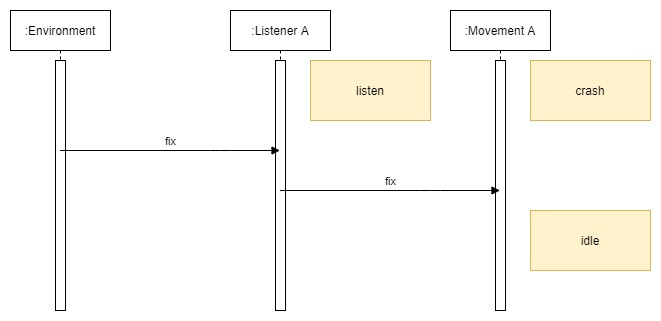
\includegraphics[width=13cm]{messaggi_macchina_fixcar.jpg}
	\caption{Messaggio per la riparazione del taxi.}
	\label{fig:messaggi_macchina_fixcar}
\end{figure}

\begin{figure}[htbp]
	\centering
	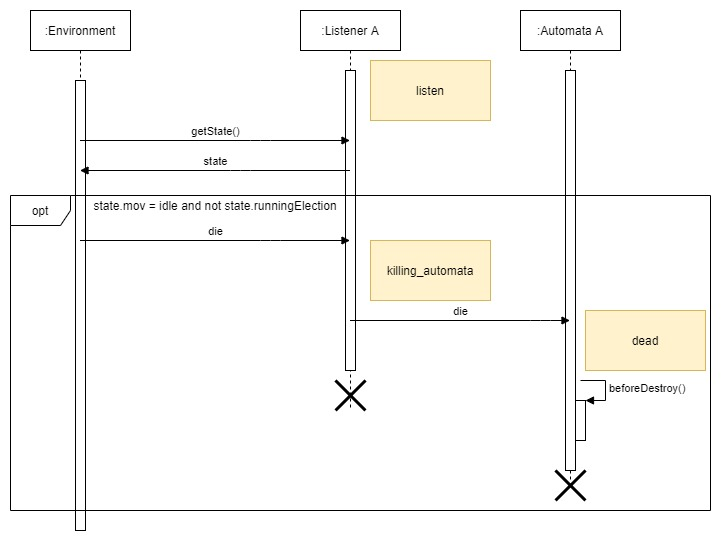
\includegraphics[width=13cm]{messaggi_macchina_rimozione.jpg}
	\caption{Messaggi inviati per la rimozione di un taxi.}
	\label{fig:messaggi_macchina_rimozione}
\end{figure}

\chapter{Test Effettuati} \label{test_log_appendix}

\section{Tre utenti e una macchina} \label{tre_utenti_una_macchina_test}
\begin{lstlisting}
4> environment:spawnCars(PID_ENV, 1).
{spawn,cars,1}
5> ["Car"] {"c1"} - Car ready in position ["f"]
5> environment:spawnUsers(PID_ENV, 3).
{spawn,users,3}
6> ["User"] {"u1"} - I'm a new user, i'm going from ["i"] to ["h"]
6> ["User"] {"u2"} - I'm a new user, i'm going from ["e"] to ["a"]
6> ["User"] {"u3"} - I'm a new user, i'm going from ["b"] to ["g"]
6> ["User"] {"u2"} - "App_User - Nearest Taxi is already running election."
6> ["User"] {"u3"} - "App_User - Nearest Taxi is already running election."
6> ["Car"] {"c1"} - Car Stops for client: ["i","h"] | Total Time for client: 26
6> ["User"] {"u1"} - Taxi ["c1"] is serving me with 20 time to wait
6> ["User"] {"u3"} - "App_User - Waited random time, going back to begin election"
6> ["Car"] {"c1"} - Car Stops for client: ["b","f","g"] | Total Time for client: 63
6> ["User"] {"u3"} - Taxi ["c1"] is serving me with 39 time to wait
6> ["User"] {"u2"} - "App_User - Waited random time, going back to begin election"
6> ["User"] {"u2"} - "App_User - No taxi has won election running election."
6> ["User"] {"u1"} - Taxi ["c1"] is arrived in my position!
6> ["User"] {"u2"} - "App_User - Waited random time, going back to begin election"
6> ["User"] {"u2"} - "App_User - No taxi has won election running election."
6> ["User"] {"u2"} - "App_User - Waited random time, going back to begin election"
6> ["User"] {"u2"} - "App_User - No taxi has won election running election."
6> ["Car"] {"c1"} - Arrived in user target position ["h"]
6> ["User"] {"u1"} - I'm arrived in my target position ["h"]
6> ["User"] {"u1"} - "I made my trip, goodbye."
6> ["User"] {"u2"} - "App_User - Waited random time, going back to begin election"
6> ["User"] {"u2"} - "App_User - No taxi has won election running election."
6> ["User"] {"u3"} - Taxi ["c1"] is arrived in my position!
6> ["User"] {"u2"} - "App_User - Waited random time, going back to begin election"
6> ["User"] {"u2"} - "App_User - No taxi has won election running election."
6> ["Car"] {"c1"} - Arrived in user target position ["g"]
6> ["User"] {"u3"} - I'm arrived in my target position ["g"]
6> ["User"] {"u3"} - "I made my trip, goodbye."
6> ["User"] {"u2"} - "App_User - Waited random time, going back to begin election"
6> ["User"] {"u2"} - "App_User - No taxi has won election running election."
6> ["Car"] {"c1"} - "Battery - Triggered Solar Charging"
6> ["User"] {"u2"} - "App_User - Waited random time, going back to begin election"
6> ["User"] {"u2"} - "App_User - No taxi has won election running election."
6> ["User"] {"u2"} - "App_User - Waited random time, going back to begin election"
6> ["User"] {"u2"} - "App_User - No taxi has won election running election."
6> ["User"] {"u2"} - "App_User - Waited random time, going back to begin election"
6> ["Car"] {"c1"} - Car Stops for client: ["c","e","a"] | Total Time for client: 44
6> ["User"] {"u2"} - Taxi ["c1"] is serving me with 26 time to wait
6> ["User"] {"u2"} - Taxi ["c1"] is arrived in my position!
6> ["Car"] {"c1"} - "Battery - Level under minimum value"
6> ["Car"] {"c1"} - Low battery, enable path to charging: ["d","c"]
6> ["Car"] {"c1"} - Arrived in user target position ["a"]
6> ["User"] {"u2"} - I'm arrived in my target position ["a"]
6> ["User"] {"u2"} - "I made my trip, goodbye."
6> ["Car"] {"c1"} - I'm in charging column position, recharging. Current level: 0
6> ["Car"] {"c1"} - "Battery - Level over minimum"
6> ["Car"] {"c1"} - "Battery - Level maximum"
\end{lstlisting}

\section{Un utente più macchine}\label{log_one_user_more_cars}
\begin{lstlisting}
7> environment:printCars(PID_ENV).
["Env"] {<0.219.0>} - Cars in city: ["c4","c1","c5","c2","c3"]
{print,self,cars}
8> environment:spawnUsers(PID_ENV, 1).
{spawn,users,1}
["User"] {"u4"} - I'm a new user, i'm going from ["d"] to ["e"]
9> ["Car"] {"c1"} - Car Stops for client: ["d","c","e"] | Total Time for client: 25
9> ["User"] {"u4"} - Taxi ["c1"] is serving me with 6 time to wait
9> ["User"] {"u4"} - Taxi ["c1"] is arrived in my position!
9> ["Car"] {"c1"} - Arrived in user target position ["e"]
9> ["User"] {"u4"} - I'm arrived in my target position ["e"]
9> ["User"] {"u4"} - "I made my trip, goodbye."
\end{lstlisting}

\section{Evento Cambia Destinazione}\label{log_change_dest}
\begin{lstlisting}
13> environment:spawnCars(PID_ENV, 1).
{spawn,cars,1}
["Car"] {"c1"} - Car ready in position ["b"]
14> environment:spawnUsers(PID_ENV, 1).
{spawn,users,1}
["User"] {"u1"} - I'm a new user, i'm going from ["i"] to ["d"]
15> ["Car"] {"c1"} - Car Stops for client: ["e","i","d"] | Total Time for client: 38
15> ["User"] {"u1"} - Taxi ["c1"] is serving me with 19 time to wait
15> environment:triggerEvent(PID_ENV, 3).
["Env"] {<0.286.0>} - Event: "client change target"
{event,3}
16> ["Car"] {"c1"} - Car Stops for client: ["i","h"] | Total Time for client: 21
16> ["User"] {"u1"} - I'm successfully changed my target position to ["h"]
16> ["User"] {"u1"} - Taxi ["c1"] is arrived in my position!
16> ["Car"] {"c1"} - Arrived in user target position ["h"]
16> ["User"] {"u1"} - I'm arrived in my target position ["h"]
16> ["User"] {"u1"} - "I made my trip, goodbye."
\end{lstlisting}

\section{Evento Car crash e Fix car} \label{car_crash_fix_event}
\begin{lstlisting}
["User"] {"u3"} - "App_User - Nearest Taxi is already running election." 
["Car"] {"c1"} - Car Stops for client: ["i","h"] | Total Time for client: 12
["User"] {"u1"} - Taxi ["c1"] is serving me with 6 time to wait
["User"] {"u3"} - "App_User - Waited random time, going back to begin election" 
["Car"] {"c1"} - Car Stops for client: ["i","f"] | Total Time for client: 36
["User"] {"u3"} - Taxi ["c1"] is serving me with 16 time to wait
["User"] {"u2"} - "App_User - Waited random time, going back to begin election" 
["Car"] {"c1"} - Car Stops for client: ["a","f","h"] | Total Time for client: 75
["User"] {"u2"} - Taxi ["c1"] is serving me with 48 time to wait
["User"] {"u1"} - Taxi ["c1"] is arrived in my position!
["User"] {"u1"} - I'm arrived in my target position ["h"]
["User"] {"u1"} - "I made my trip, goodbye." 
environment:triggerEvent(PID_ENV, 4).
["Env"] {<0.378.0>} - Event: "car crash"
["Env"] {<0.378.0>} - Car with name {"c1"} has punctured rubber of the car!
["Car"] {"c1"} - "I am broken, now i notify my users and waiting for fix" 
{event,4}
["User"] {"u2"} - "App_User - Car Crashed" 
["User"] {"u3"} - "App_User - Car Crashed" 
22> ["User"] {"u3"} - "App_User - Waited random time after car crashed, going back to begin election" 
["User"] {"u2"} - "App_User - Waited random time after car crashed, going back to begin election" 
["User"] {"u2"} - "App_User - No taxi has won election running election." 
["User"] {"u3"} - "App_User - Waited random time, going back to begin election" 
["User"] {"u3"} - "App_User - No taxi has won election running election." 
environment:triggerEvent(PID_ENV, 5).
["Env"] {<0.378.0>} - Event: "fix car"
["Env"] {<0.378.0>} - Car with name {"c1"} has been fixed!
{event,5}
["Car"] {"c1"} - "I am fixed, now I can serve again" 
23> ["User"] {"u3"} - "App_User - Waited random time, going back to begin election" 
["Car"] {"c1"} - Car Stops for client: ["i","f"] | Total Time for client: 26
["User"] {"u3"} - Taxi ["c1"] is serving me with 6 time to wait
["User"] {"u2"} - "App_User - Waited random time, going back to begin election" 
["Car"] {"c1"} - Car Stops for client: ["a","f","h"] | Total Time for client: 63
["User"] {"u2"} - Taxi ["c1"] is serving me with 36 time to wait
["User"] {"u3"} - Taxi ["c1"] is arrived in my position!
\end{lstlisting}